% Required packages in the main paper preamble:
% \usepackage{booktabs}

\section{I INTRODUCTION}

Modern medical artificial intelligence is increasingly developed in a multi-center environment. A useful diagnostic model may require information from several hospitals, scanners, departments, and patient populations, but these participants are rarely synchronized. In practice, hospitals finish local training at different times, use devices with different imaging characteristics, and observe different subsets of the diagnostic label space. For example, a hematology center may contain abundant common blood-cell categories but very limited rare cell types, while an ultrasound center may be dominated by a small number of routine findings. These constraints motivate one-shot asynchronous medical model merging: after local training, each hospital uploads once, and a server constructs a global diagnostic model without iterative communication.

This setting is different from federated learning. Federated optimization assumes repeated rounds of server aggregation, client-side continued training, and re-uploaded updates. Such a protocol is expensive and often unrealistic when clients are asynchronous, offline, or unwilling to participate in repeated training rounds. Our setting is also different from standard post-hoc model merging in natural language processing, where models are usually fine-tuned from the same foundation model on semantically rich tasks with broad label coverage. In medical imaging, client data are often label-incomplete and long-tailed: each client can be locally meaningful, but no single client necessarily covers the entire diagnostic space.

A direct application of existing post-hoc merging algorithms exposes a failure mode that is easy to miss if only accuracy is considered. We observe aggregation-induced predictive collapse: local medical models may still predict multiple categories before merging, but many parameter-space merging rules turn the merged model into a single-class or few-class predictor. On our diagnostic probe, generic merging baselines excluding LAMP-Merge obtain an average collapse ratio of 0.7993 and use only 1.8600 effective predicted classes. Standard averaging alone has a collapse ratio of 0.8028. In contrast, a natural-image CIFAR-10 partial-label control with standard averaging remains non-collapsed, with a collapse ratio of 0.2425 and 10.0000 effective predicted classes. This suggests that medical long-tailed class priors and incomplete local diagnostic coverage amplify a distinct post-hoc merging failure mode.

We propose LAMP-Merge, a Long-tail-Aware Medical Prototype merging framework for asynchronous medical model merging. LAMP-Merge keeps the communication one-shot and does not require the server to access raw medical images. Each client computes class-level diagnostic statistics locally and uploads only the checkpoint interface information, class support counts, class prevalence counts, and reference-backbone class prototypes. The first module reconstructs a global diagnostic prototype head in a shared reference feature space, preserving per-class local expertise rather than averaging incompatible classifier heads. The second module applies bounded long-tail prevalence calibration when the uploaded class prevalence indicates a dominant diagnosis class. This design follows two empirical observations: post-hoc merging induces predictive collapse in medical images, and, under strongly long-tailed medical priors, collapse can appear beneficial in accuracy because the majority class itself occupies a large portion of the test distribution.

Our contributions are summarized as follows. First, we formulate a one-shot asynchronous medical model merging problem that is distinct from federated learning and from data-free NLP-style model merging. Second, we identify predictive collapse as a central failure mode of generic merging algorithms under incomplete local diagnostic coverage. Third, we introduce LAMP-Merge, which uses client-side class prototypes and prevalence counts to reconstruct a non-collapsed global diagnostic model without exposing raw images. Fourth, we provide a broad empirical study over five medical image datasets, five model families, three client counts, and three non-IID skew levels; LAMP-Merge wins or ties the strongest non-LAMP baseline in 68 out of 75 client-average cells.

\section{II RELATED WORKS}

\subsection{Post-hoc Model Merging}

Post-hoc model merging aims to combine independently trained checkpoints without the full cost of joint training. Weight averaging and model soups average parameters directly and can be effective when models remain in a compatible basin~\cite{wortsman2022model}. Task arithmetic represents fine-tuned models as parameter deltas relative to a shared initialization and combines these deltas linearly~\cite{ilharco2023task}. Git Re-Basin studies permutation symmetries and aligns neurons before averaging~\cite{ainsworth2023git}. TIES-Merging and DARE-style methods further address interference by trimming small updates, resolving sign conflicts, or dropping and rescaling task vectors~\cite{yadav2023ties,yu2024dare}. RegMean, Fisher merging, Model Stock, Breadcrumbs, Iso-C, FreeMerge, and RobustMerge introduce additional geometric, curvature, or robustness assumptions for parameter-space fusion~\cite{matena2022fisher,jin2023regmean}.

These methods are important baselines, but their assumptions do not directly address the medical setting studied here. Most are class-agnostic at the diagnostic level: they manipulate parameters, task vectors, curvature estimates, or update signs without asking which client actually has reliable evidence for each medical class. Under local class incompleteness, this can turn several locally meaningful classifiers into a globally collapsed classifier. Our prediction-distribution analysis confirms this failure: generic merging baselines often preserve a dominant class direction while suppressing rare or locally missing diagnosis classes, leading to low balanced accuracy and macro F1 even when raw accuracy is sometimes high. Therefore, the limitation is not simply that these baselines are weak; rather, their fusion variables are misaligned with the central structure of multi-center medical data, namely class-dependent diagnostic availability and long-tailed prevalence.

\subsection{Federated and Decentralized Medical Learning}

Federated learning and decentralized learning are widely studied for privacy-sensitive medical AI. Federated averaging and its variants train a global model through repeated communication rounds. Swarm learning removes the central parameter server and relies on decentralized coordination~\cite{warnat2021swarm}, while gossip-style learning propagates models asynchronously among participants. These approaches are valuable when clients can repeatedly train, communicate, and update their models.

Our problem is intentionally narrower and stricter in communication. We consider one-shot post-hoc merging after local training has already finished. The server does not send a sequence of global models back to clients, and clients do not perform multi-round optimization in response to server updates. Therefore, federated and decentralized training protocols are not direct solutions for our setting. They solve collaborative training, whereas we solve asynchronous diagnostic model fusion with a single upload event.

\subsection{Medical Fusion and Multimodal Clinical Modeling}

Medical fusion methods often exploit modality-specific structure. Examples include irregularly sampled clinical time-series fusion, continuous-time attention for clinical observations, graph-based physiological sensor fusion, and image-EHR fusion such as chest X-ray plus clinical time-series models~\cite{shukla2021mtan,zhang2022raindrop,hayat2022medfuse}. These methods demonstrate that medical data have distinctive temporal, modality, and prevalence structures. However, they normally assume access to patient-level samples, synchronized multimodal records, or server-side validation data during model learning. They are not designed to merge independently trained image classifiers when the server cannot inspect raw medical images.

This gap motivates our design. Existing medical fusion algorithms show the value of clinical structure, but they do not satisfy one-shot asynchronous checkpoint merging. Existing post-hoc merging algorithms satisfy the one-shot requirement, but they are not diagnostic-class aware and collapse under medical long-tail partitions. Thus, under the joint constraints of medical specificity, one-shot asynchronous merging, and no server-side raw images, existing methods are not directly applicable. LAMP-Merge combines these requirements by using only client-uploaded class-level statistics: diagnostic prototypes and prevalence counts.

\subsection{Medical Model Merging}

Recent medical model merging studies further confirm that medical imaging requires domain-specific fusion variables, but they do not satisfy the same protocol as ours. FedSoup is a personalized federated learning method: each client maintains a global model pool during federated training and selects local/global interpolations for personalization~\cite{chen2023fedsoup}. It is not a one-shot post-hoc merger that outputs a single shared checkpoint; if the personalized soups are averaged again into one global model, site-adapted feature and normalization statistics can be mixed a second time, aggravating medical site shift. MedMerge learns kernel-level fusion weights for target-domain transfer from different initializations~\cite{almakky2024medmerge}. It is designed for a target task with target-domain optimization, rather than a single asynchronous aggregation of same-task client checkpoints with incomplete local label coverage. FissionFusion generates multiple fine-tuned models and uses hierarchical souping selected by validation performance~\cite{sanjeev2024fissionfusion}; this is a strong medical souping framework, but its selection stage assumes access to validation feedback and model-generation trajectories outside our one-upload setting. MedSAMix merges SAM-based generalist and specialist segmenters with zero-order layer-wise optimization for medical segmentation~\cite{yang2026medsamix}; it targets foundation segmentation models and optimization regimes, not class-skewed diagnostic classifier checkpoints. InMerge merges similar kernels within a single model during fine-tuning~\cite{wang2025inmerge}, so it is a regularization method rather than inter-client checkpoint fusion.

These methods are therefore complementary but not direct solutions. A recurring issue is where model selection or fusion-weight estimation is performed. If validation images, target-domain images, or empirical task feedback are centralized at the server, the protocol violates our server-side privacy boundary. If the same evaluation is sent back to clients, the method no longer remains a one-shot post-hoc merger; it becomes an additional client-feedback protocol whose communication pattern is closer to federated learning. Some methods also require explicit federated model-pool communication, while others operate within a single model rather than across clients. LAMP-Merge instead keeps the server-side operation one-shot and constructs the shared diagnostic model only from uploaded checkpoints and class-level medical statistics.

\section{III LAMP FRAMEWORK}

\subsection{Problem Formulation}

Assume $K$ medical clients. Client $i$ owns a private labeled dataset $D_i=\{(x,y)\}$ drawn from a class-skewed medical distribution over $C$ diagnosis classes. Each client trains a local model independently and asynchronously. After local training, the client performs one upload containing the model interface and class-level diagnostic statistics computed locally. The server must produce one global model in a single post-hoc merging step. The server cannot access raw medical images, sample-level features, sample-level logits, or sample-level predictions.

The key difficulty is incomplete local diagnostic coverage. Let $D_{i,c}$ denote the subset of client $i$ belonging to diagnosis class $c$. In medical partitions, $D_{i,c}$ can be empty for many classes. Thus, a client can be reliable for a subset of diagnoses but unreliable for unseen classes. A class-agnostic parameter merge has no explicit mechanism to preserve this local reliability structure.

\subsection{Observation 1: Aggregation-induced Predictive Collapse}

Before introducing the algorithm, we formalize the diagnostic quantity used to identify collapse. For a model evaluated on $N$ test images, let
\[
q(c)=\frac{1}{N}\sum_{n=1}^{N}\mathbf{1}[\hat y_n=c]
\]
be the predicted class distribution. We define the collapse ratio as
\[
\rho=\max_c q(c).
\]
A model with $\rho$ close to one behaves like a single-class predictor.

Our first observation is aggregation-induced predictive collapse: in local-class-coverage medical settings, post-hoc parameter merging can transform multiple non-degenerate local predictors into a globally collapsed predictor. The local clients may be biased because they see only part of the diagnostic space, but they can still respond to multiple classes. The collapse mainly appears after class-agnostic aggregation, where parameter averaging, sign voting, or pruning amplifies locally dominant directions without preserving per-class evidence.

\subsection{Observation 2: Collapse Benefit under Long-tailed Priors}

Our second observation is that collapse can be deceptively useful under long-tailed medical priors. Let
\[
p_{\max}=\max_c P(y=c)
\]
be the highest test-set class prior. A model that always predicts the most frequent class obtains
\[
\mathrm{Acc}_{\mathrm{collapse}}=p_{\max}.
\]
Therefore, when the most common diagnosis occupies a large fraction of the distribution, a collapsed predictor may achieve high accuracy without real multi-class diagnostic ability. This explains why some baselines can look competitive in raw accuracy while failing balanced accuracy, macro F1, and prediction-distribution diagnostics. A useful medical merging method should avoid losing rare-class discrimination, while still respecting genuine prevalence information when the task is strongly long-tailed.

\subsection{M1: Diagnostic Prototype Reconstruction}

LAMP-Merge first reconstructs a class-wise diagnostic head in a shared reference feature space. Let $\phi_0$ be the frozen reference backbone instantiated from the shared model configuration before local training, and let $T(\cdot)$ be the evaluation transform. For each diagnosis class $c$, client $i$ computes a reference-space class prototype
\[
\mu_{i,c}=\frac{1}{n_{i,c}}\sum_{(x,y)\in D_i}\mathbf{1}[y=c]\phi_0(T(x)),
\]
where $n_{i,c}=|D_{i,c}|$ is the class support count. If $n_{i,c}=0$, the client uploads zero support for that class and contributes no prototype evidence.

The server converts support counts into evidence weights:
\[
e_{i,c}=(n_{i,c}+1)^\gamma \mathbf{1}[n_{i,c}>0],
\]
where $\gamma=0.45$ is the default evidence exponent. The normalized reliability of client $i$ for class $c$ is
\[
\alpha_{i,c}=\frac{e_{i,c}}{\sum_{j=1}^{K} e_{j,c}}.
\]
The global diagnosis prototype is then
\[
p_c=\sum_{i=1}^{K}\alpha_{i,c}\mu_{i,c}.
\]
Finally, LAMP-Merge synthesizes a cosine prototype classifier:
\[
w_c=s\frac{p_c}{\|p_c\|_2},
\]
where $s=20$ is the default head scale. This module directly addresses Observation 1: instead of averaging incompatible classifier heads, it preserves the classes for which each client has evidence and reconstructs a global multi-class diagnostic head.

\subsection{M2: Long-tail Prevalence Calibration}

M1 prevents class-agnostic aggregation from collapsing the classifier, but medical tasks may contain real long-tailed prevalence. To account for Observation 2, each client also uploads class prevalence counts $m_{i,c}$. The server estimates the global class prior
\[
\pi_c=\frac{\sum_{i=1}^{K}m_{i,c}}{\sum_{k=1}^{C}\sum_{i=1}^{K}m_{i,k}}.
\]
We measure dominant-class imbalance by
\[
r=C\max_c \pi_c.
\]
M2 is activated only when $r>\tau$, where $\tau=2.5$ by default. When activated, it adds a centered log-prior bias
\[
b_c=\lambda\left(\log\pi_c-\frac{1}{C}\sum_{k=1}^{C}\log\pi_k\right),
\]
with default maximum calibration strength $\lambda=6.0$. The final score is
\[
\mathrm{score}_c(x)=w_c^\top\phi_0(T(x))+b_c.
\]
The bias is centered, bounded, and attached to the prototype classifier; it calibrates prevalence without replacing the multi-class diagnostic directions reconstructed by M1.

\section{IV EXPERIMENTS}

\subsection{Experimental Setup}

We evaluate LAMP-Merge under one-shot asynchronous medical model merging. Each client trains locally on its private class-skewed partition. After local training, it uploads one checkpoint and the class-level statistics required by LAMP-Merge. The server merges once and does not run iterative server-client optimization.

\subsubsection{Datasets}

We use five 224-resolution medical image classification datasets. All tasks are single-label multi-class diagnosis or organ recognition tasks. The exact statistics are shown in Table~\ref{tab:dataset-stats}.

\begin{table}[t]
\centering
\caption{Dataset statistics used in the experiments.}
\label{tab:dataset-stats}
\scriptsize
\setlength{\tabcolsep}{3.2pt}
\begin{tabular}{lrrrrr}
\toprule
Dataset & Classes & Channels & Train & Val & Test \\
\midrule
Blood & 8 & 3 & 11959 & 1712 & 3421 \\
Derma & 7 & 3 & 7007 & 1003 & 2005 \\
Organ-C & 11 & 1 & 12975 & 2392 & 8216 \\
Organ-S & 11 & 1 & 13932 & 2452 & 8827 \\
Ultrasound & 8 & 3 & 3869 & 549 & 1113 \\
\midrule
Total & -- & -- & 49742 & 8108 & 23582 \\
\bottomrule
\end{tabular}
\end{table}

For standard vision backbones, we evaluate ResNet, ConvNeXt, ViT-Tiny, and Swin-Tiny. For vision-language models, we evaluate \texttt{openai/clip-vit-base-patch32}. For each dataset-model pair, we construct non-IID client partitions with $K\in\{3,5,7\}$ clients and Dirichlet skew parameter $\beta\in\{0,0.01,0.1\}$. All results use seed 42. The benchmark contains 225 raw test-accuracy cells and 75 client-average cells. The client-average metric averages the three $\beta$ values for each fixed client number, reducing sensitivity to a single partition skew.

\subsubsection{Baselines}

We compare with twelve post-hoc merging baselines: \texttt{avg}, \texttt{ties}, \texttt{dare\_linear}, \texttt{dare\_ties}, \texttt{regmean}, \texttt{fisher}, \texttt{breadcrumbs}, \texttt{model\_stock}, \texttt{from}, \texttt{iso\_c}, \texttt{free\_merge}, and \texttt{robustmerge}. The main comparison counts a cell as successful when LAMP-Merge is greater than or equal to the strongest non-LAMP baseline in that cell.

\subsection{Experiment Environment}

All experiments were run on a server with two Intel(R) Xeon(R) Silver 4210 CPUs @ 2.20GHz, 40 logical CPU threads in total, and four NVIDIA GeForce RTX 2080 Ti GPUs with 11264 MiB memory each. The NVIDIA driver version is 535.154.05. The operating system is Ubuntu 20.04.1 LTS. The software environment is the conda environment \texttt{MM}, using Python 3.10.20, PyTorch 2.6.0+\texttt{cu118}, torchvision 0.21.0+\texttt{cu118}, NumPy 2.2.6, and CUDA runtime 11.8.

\subsection{Hyperparameter Settings}

Unless otherwise stated, LAMP-Merge uses evidence exponent $\gamma=0.45$, prototype head scale $s=20$, long-tail activation threshold $\tau=2.5$, and prevalence calibration strength $\lambda=6.0$. These hyperparameters are fixed for all datasets, backbones, client counts, and skew levels.

\subsection{Main Client-average Results}

Tables~\ref{tab:client-avg-resnet}--\ref{tab:client-avg-openai-clip-vit-base-patch32} report all client-average results from the full benchmark. Across the 75 client-average cells, LAMP-Merge wins or ties the strongest non-LAMP baseline in 68 cells, corresponding to 90.7\%. Across all 300 cells including raw and client-average entries, LAMP-Merge wins or ties in 241 cells.

\begin{table*}[t]
\centering
\scriptsize
\setlength{\tabcolsep}{2.6pt}
\caption{Client-average test accuracy on resnet. Each entry averages the three Dirichlet settings for a fixed client number.}
\label{tab:client-avg-resnet}
\begin{tabular}{lccccccccccccccc}
\toprule
& \multicolumn{3}{c}{Blood} & \multicolumn{3}{c}{Derma} & \multicolumn{3}{c}{Organ-C} & \multicolumn{3}{c}{Organ-S} & \multicolumn{3}{c}{Ultrasound} \\
\cmidrule(lr){2-4}\cmidrule(lr){5-7}\cmidrule(lr){8-10}\cmidrule(lr){11-13}\cmidrule(lr){14-16}
Method & $K=3$ & $K=5$ & $K=7$ & $K=3$ & $K=5$ & $K=7$ & $K=3$ & $K=5$ & $K=7$ & $K=3$ & $K=5$ & $K=7$ & $K=3$ & $K=5$ & $K=7$ \\
\midrule
\texttt{avg} & 0.3345 & 0.2467 & 0.2822 & 0.6291 & 0.4700 & 0.6244 & 0.2261 & 0.1772 & 0.1396 & \underline{0.2864} & 0.1794 & 0.2475 & 0.2435 & 0.1581 & 0.1542 \\
\texttt{ties} & 0.2601 & 0.1872 & 0.1787 & 0.5995 & 0.4841 & 0.6484 & 0.2650 & 0.1684 & \underline{0.2118} & 0.1981 & 0.1915 & 0.1874 & \underline{0.3477} & 0.1989 & 0.1854 \\
\texttt{dare\_linear} & 0.2832 & \underline{0.2856} & 0.2392 & 0.6357 & 0.4841 & 0.6288 & 0.2018 & \underline{0.2588} & 0.1650 & 0.2545 & 0.2245 & \underline{0.2537} & 0.2162 & 0.1728 & 0.1608 \\
\texttt{dare\_ties} & 0.3194 & 0.1935 & 0.1780 & 0.5375 & 0.4825 & 0.5558 & 0.1851 & 0.1515 & 0.1859 & 0.1790 & 0.1352 & 0.1730 & 0.2932 & 0.1635 & 0.1890 \\
\texttt{regmean} & \underline{0.3460} & 0.2369 & \underline{0.3407} & 0.5812 & 0.2843 & 0.5022 & 0.2405 & 0.1340 & 0.1388 & 0.2504 & 0.1623 & 0.1493 & 0.2276 & 0.1695 & 0.1318 \\
\texttt{fisher} & 0.3196 & 0.2237 & 0.2608 & 0.6707 & \underline{0.6702} & \underline{0.6690} & \underline{0.2973} & 0.1741 & 0.1812 & 0.2010 & \underline{0.2956} & 0.1963 & 0.2333 & 0.1860 & \underline{0.2513} \\
\texttt{breadcrumbs} & 0.0854 & 0.1417 & 0.1460 & 0.0495 & 0.2913 & 0.1721 & 0.0766 & 0.0676 & 0.0685 & 0.0802 & 0.0948 & 0.0603 & 0.1225 & 0.1273 & 0.1021 \\
\texttt{model\_stock} & 0.2420 & 0.1824 & 0.1975 & 0.6216 & 0.4311 & 0.5721 & 0.1225 & 0.1274 & 0.1185 & 0.2742 & 0.1578 & 0.2012 & 0.1791 & 0.1321 & 0.1578 \\
\texttt{from} & 0.2989 & 0.2306 & 0.2052 & \underline{0.6713} & 0.4369 & 0.6580 & 0.2350 & 0.1560 & 0.1520 & 0.2207 & 0.2087 & 0.2476 & 0.2309 & 0.1506 & 0.2063 \\
\texttt{iso\_c} & 0.3278 & 0.2748 & 0.3023 & 0.5049 & 0.4422 & 0.6416 & 0.2331 & 0.1629 & 0.1383 & 0.2736 & 0.2118 & 0.2453 & 0.2615 & 0.1698 & 0.1554 \\
\texttt{free\_merge} & 0.3345 & 0.2467 & 0.2822 & 0.6291 & 0.4700 & 0.6246 & 0.2261 & 0.1771 & 0.1396 & 0.2863 & 0.1793 & 0.2475 & 0.2435 & 0.1581 & 0.1545 \\
\texttt{robustmerge} & 0.3401 & 0.2430 & 0.2256 & 0.2956 & 0.2085 & 0.3942 & 0.2458 & 0.1764 & 0.1653 & 0.2680 & 0.2227 & 0.2301 & 0.2189 & \underline{0.2231} & 0.1707 \\
\textbf{LAMP-Merge} & \textbf{0.8002} & \textbf{0.7999} & \textbf{0.8007} & \textbf{0.6745} & \textbf{0.6761} & \textbf{0.6763} & \textbf{0.6074} & \textbf{0.6069} & \textbf{0.6076} & \textbf{0.5531} & \textbf{0.5524} & \textbf{0.5517} & \textbf{0.4762} & \textbf{0.4762} & \textbf{0.4762} \\
\bottomrule
\end{tabular}
\end{table*}

\begin{table*}[t]
\centering
\scriptsize
\setlength{\tabcolsep}{2.6pt}
\caption{Client-average test accuracy on convnext. Each entry averages the three Dirichlet settings for a fixed client number.}
\label{tab:client-avg-convnext}
\begin{tabular}{lccccccccccccccc}
\toprule
& \multicolumn{3}{c}{Blood} & \multicolumn{3}{c}{Derma} & \multicolumn{3}{c}{Organ-C} & \multicolumn{3}{c}{Organ-S} & \multicolumn{3}{c}{Ultrasound} \\
\cmidrule(lr){2-4}\cmidrule(lr){5-7}\cmidrule(lr){8-10}\cmidrule(lr){11-13}\cmidrule(lr){14-16}
Method & $K=3$ & $K=5$ & $K=7$ & $K=3$ & $K=5$ & $K=7$ & $K=3$ & $K=5$ & $K=7$ & $K=3$ & $K=5$ & $K=7$ & $K=3$ & $K=5$ & $K=7$ \\
\midrule
\texttt{avg} & 0.1565 & 0.1122 & 0.1384 & 0.2966 & \underline{0.4830} & \textbf{0.6688} & 0.1037 & 0.1218 & 0.0944 & 0.1308 & 0.1035 & 0.1416 & 0.1506 & 0.1506 & 0.1252 \\
\texttt{ties} & 0.1715 & 0.1214 & 0.1524 & 0.2966 & 0.1797 & 0.2713 & 0.1217 & 0.0786 & 0.0716 & 0.1123 & 0.0761 & 0.0796 & 0.1518 & 0.1456 & 0.1291 \\
\texttt{dare\_linear} & 0.1756 & 0.1122 & 0.1345 & 0.2705 & \underline{0.4830} & 0.4830 & 0.1035 & 0.0699 & 0.1085 & 0.1282 & 0.1035 & 0.0797 & 0.1575 & 0.1575 & 0.1264 \\
\texttt{dare\_ties} & 0.1096 & 0.1519 & 0.1497 & 0.0908 & 0.2798 & 0.2451 & 0.1305 & 0.1346 & 0.0770 & 0.1096 & 0.0946 & 0.0709 & 0.1456 & 0.1297 & 0.1500 \\
\texttt{regmean} & 0.1565 & 0.0817 & \underline{0.1856} & 0.2633 & 0.0773 & 0.2720 & 0.1143 & 0.1017 & 0.0768 & 0.1014 & 0.1259 & 0.1038 & 0.1575 & 0.1539 & 0.1500 \\
\texttt{fisher} & 0.1565 & 0.0999 & 0.1189 & \underline{0.4825} & 0.2638 & 0.2971 & 0.1003 & 0.0974 & 0.0915 & 0.0604 & 0.0517 & 0.0843 & \underline{0.1695} & 0.1360 & 0.1456 \\
\texttt{breadcrumbs} & 0.1516 & 0.1366 & 0.1163 & 0.0524 & 0.2766 & 0.4630 & 0.1031 & \underline{0.1444} & 0.1574 & 0.1516 & \underline{0.1554} & \underline{0.2077} & 0.1384 & 0.1363 & 0.1363 \\
\texttt{model\_stock} & 0.1756 & 0.1144 & 0.1778 & 0.2966 & \underline{0.4830} & \textbf{0.6688} & 0.1276 & 0.1218 & 0.1385 & 0.1308 & 0.1035 & 0.1935 & 0.1575 & 0.1291 & 0.1479 \\
\texttt{from} & 0.1565 & 0.1083 & 0.1671 & 0.2966 & 0.3406 & 0.4569 & 0.1232 & 0.1224 & 0.0650 & 0.1324 & 0.1105 & 0.0897 & 0.1575 & \underline{0.1578} & 0.1087 \\
\texttt{iso\_c} & \underline{0.1947} & \underline{0.1865} & 0.1480 & 0.2971 & \underline{0.4830} & \textbf{0.6688} & 0.0991 & 0.0699 & 0.0945 & 0.0789 & 0.1477 & 0.0867 & 0.1518 & 0.1291 & 0.1605 \\
\texttt{free\_merge} & 0.1575 & 0.1190 & 0.1384 & 0.2971 & \underline{0.4830} & \textbf{0.6688} & 0.0906 & 0.1218 & 0.1385 & 0.1308 & 0.1035 & 0.1416 & 0.1506 & 0.1291 & \underline{0.1695} \\
\texttt{robustmerge} & 0.1410 & 0.1405 & 0.0752 & 0.0908 & 0.4507 & 0.4830 & \underline{0.1394} & 0.1218 & \underline{0.1793} & \underline{0.2354} & 0.0961 & \underline{0.2077} & 0.1300 & 0.1135 & 0.1363 \\
\textbf{LAMP-Merge} & \textbf{0.8482} & \textbf{0.8483} & \textbf{0.8493} & \textbf{0.5992} & \textbf{0.5920} & \underline{0.5852} & \textbf{0.6482} & \textbf{0.6480} & \textbf{0.6495} & \textbf{0.5977} & \textbf{0.5985} & \textbf{0.5990} & \textbf{0.4259} & \textbf{0.4259} & \textbf{0.4259} \\
\bottomrule
\end{tabular}
\end{table*}

\begin{table*}[t]
\centering
\scriptsize
\setlength{\tabcolsep}{2.6pt}
\caption{Client-average test accuracy on vit\_t. Each entry averages the three Dirichlet settings for a fixed client number.}
\label{tab:client-avg-vit-t}
\begin{tabular}{lccccccccccccccc}
\toprule
& \multicolumn{3}{c}{Blood} & \multicolumn{3}{c}{Derma} & \multicolumn{3}{c}{Organ-C} & \multicolumn{3}{c}{Organ-S} & \multicolumn{3}{c}{Ultrasound} \\
\cmidrule(lr){2-4}\cmidrule(lr){5-7}\cmidrule(lr){8-10}\cmidrule(lr){11-13}\cmidrule(lr){14-16}
Method & $K=3$ & $K=5$ & $K=7$ & $K=3$ & $K=5$ & $K=7$ & $K=3$ & $K=5$ & $K=7$ & $K=3$ & $K=5$ & $K=7$ & $K=3$ & $K=5$ & $K=7$ \\
\midrule
\texttt{avg} & 0.1343 & 0.1082 & 0.1160 & 0.4638 & 0.4369 & 0.3696 & 0.1657 & 0.1043 & 0.0952 & 0.0844 & 0.0852 & 0.1710 & 0.1450 & 0.1327 & \underline{0.1884} \\
\texttt{ties} & 0.0796 & 0.1421 & 0.1285 & 0.4780 & 0.3498 & 0.4615 & 0.1341 & 0.1223 & 0.0953 & 0.1192 & 0.1002 & 0.1597 & \underline{0.2001} & 0.1306 & 0.1018 \\
\texttt{dare\_linear} & \underline{0.2397} & 0.1129 & 0.1387 & 0.2850 & 0.1002 & 0.1204 & 0.1534 & 0.0946 & 0.0704 & 0.0748 & 0.0549 & 0.1611 & 0.1366 & 0.1051 & 0.1435 \\
\texttt{dare\_ties} & 0.0735 & 0.1189 & 0.1146 & 0.2735 & 0.4502 & 0.3528 & 0.1252 & 0.0903 & 0.1033 & 0.0541 & 0.0874 & 0.0591 & 0.1447 & 0.1120 & 0.1042 \\
\texttt{regmean} & 0.1748 & 0.1417 & 0.1290 & 0.5114 & 0.3667 & \underline{0.6658} & 0.1250 & 0.0964 & 0.0983 & \underline{0.1263} & 0.0717 & 0.1068 & 0.1491 & 0.1384 & 0.1144 \\
\texttt{fisher} & 0.1166 & \underline{0.1512} & \underline{0.1944} & 0.4780 & 0.2042 & 0.4820 & 0.0799 & 0.1072 & 0.1424 & 0.0856 & \underline{0.1218} & 0.1222 & 0.1611 & 0.1315 & 0.1420 \\
\texttt{breadcrumbs} & 0.1363 & 0.1039 & 0.1300 & 0.0489 & 0.2572 & 0.0607 & 0.0773 & 0.1000 & \underline{0.1644} & 0.1237 & 0.0483 & 0.1219 & 0.1360 & 0.1141 & 0.1524 \\
\texttt{model\_stock} & 0.1940 & 0.1120 & 0.1134 & 0.3805 & 0.3079 & 0.2735 & 0.1488 & 0.1227 & 0.1215 & 0.0893 & 0.0859 & \underline{0.1867} & 0.1599 & 0.1809 & 0.1641 \\
\texttt{from} & 0.1802 & 0.0781 & 0.1405 & 0.4695 & \underline{0.5121} & \textbf{0.6688} & \underline{0.2148} & \underline{0.1301} & 0.0972 & 0.0772 & 0.0798 & 0.1485 & 0.1836 & 0.1743 & 0.1776 \\
\texttt{iso\_c} & 0.1234 & 0.1483 & 0.1018 & \underline{0.5709} & 0.4529 & 0.2306 & 0.1084 & 0.0567 & 0.0897 & 0.0611 & 0.0531 & 0.1081 & 0.1417 & 0.1527 & 0.1869 \\
\texttt{free\_merge} & 0.1989 & 0.1457 & 0.1392 & 0.4630 & 0.4770 & 0.3855 & 0.1425 & 0.0980 & 0.0759 & 0.0727 & 0.0914 & 0.1643 & 0.1405 & 0.1593 & 0.1647 \\
\texttt{robustmerge} & 0.1482 & 0.1070 & 0.1425 & 0.0347 & 0.2768 & 0.1724 & 0.0954 & 0.0617 & 0.1438 & 0.1260 & 0.0707 & 0.1217 & 0.1698 & \underline{0.1854} & 0.1563 \\
\textbf{LAMP-Merge} & \textbf{0.8523} & \textbf{0.8522} & \textbf{0.8516} & \textbf{0.5970} & \textbf{0.5938} & 0.5860 & \textbf{0.5805} & \textbf{0.5790} & \textbf{0.5790} & \textbf{0.5406} & \textbf{0.5372} & \textbf{0.5388} & \textbf{0.4645} & \textbf{0.4645} & \textbf{0.4645} \\
\bottomrule
\end{tabular}
\end{table*}

\begin{table*}[t]
\centering
\scriptsize
\setlength{\tabcolsep}{2.6pt}
\caption{Client-average test accuracy on swin\_tiny. Each entry averages the three Dirichlet settings for a fixed client number.}
\label{tab:client-avg-swin-tiny}
\begin{tabular}{lccccccccccccccc}
\toprule
& \multicolumn{3}{c}{Blood} & \multicolumn{3}{c}{Derma} & \multicolumn{3}{c}{Organ-C} & \multicolumn{3}{c}{Organ-S} & \multicolumn{3}{c}{Ultrasound} \\
\cmidrule(lr){2-4}\cmidrule(lr){5-7}\cmidrule(lr){8-10}\cmidrule(lr){11-13}\cmidrule(lr){14-16}
Method & $K=3$ & $K=5$ & $K=7$ & $K=3$ & $K=5$ & $K=7$ & $K=3$ & $K=5$ & $K=7$ & $K=3$ & $K=5$ & $K=7$ & $K=3$ & $K=5$ & $K=7$ \\
\midrule
\texttt{avg} & 0.1565 & 0.1186 & 0.1524 & 0.4569 & \underline{0.4830} & \textbf{0.6688} & 0.1068 & 0.1294 & 0.0787 & 0.0682 & 0.0604 & 0.1381 & 0.1527 & 0.1294 & 0.1465 \\
\texttt{ties} & 0.0972 & 0.1190 & 0.1384 & 0.0841 & 0.0780 & \textbf{0.6688} & 0.1160 & 0.0702 & 0.0934 & 0.0734 & 0.0607 & 0.1107 & 0.1695 & 0.1303 & 0.1261 \\
\texttt{dare\_linear} & 0.1565 & 0.1161 & 0.1825 & 0.4569 & 0.2771 & 0.4630 & 0.1155 & 0.1272 & 0.0776 & 0.0640 & 0.0720 & 0.1381 & 0.1743 & 0.1536 & 0.1497 \\
\texttt{dare\_ties} & 0.1384 & 0.1162 & 0.1384 & 0.2961 & 0.2638 & \textbf{0.6688} & 0.1276 & 0.0774 & 0.1116 & 0.1194 & 0.0434 & 0.1230 & \underline{0.1791} & 0.1351 & 0.1300 \\
\texttt{regmean} & 0.1374 & 0.1715 & 0.1578 & 0.2705 & 0.4630 & 0.4569 & 0.1411 & 0.0773 & 0.0811 & 0.1215 & 0.0821 & 0.0926 & 0.1465 & 0.1105 & 0.1779 \\
\texttt{fisher} & \underline{0.1633} & \underline{0.1756} & 0.1565 & \underline{0.4582} & 0.0652 & 0.4718 & 0.0814 & 0.0899 & 0.0978 & 0.0651 & 0.0650 & 0.1092 & 0.1746 & 0.1165 & 0.1755 \\
\texttt{breadcrumbs} & 0.1500 & 0.1365 & 0.1537 & 0.0647 & 0.2771 & 0.0715 & 0.1445 & \underline{0.1783} & 0.1660 & \underline{0.2354} & \underline{0.2077} & \underline{0.2111} & 0.1450 & 0.1312 & 0.1653 \\
\texttt{model\_stock} & 0.1374 & 0.1440 & 0.1715 & 0.4569 & 0.2771 & 0.4825 & 0.1110 & 0.0771 & 0.1404 & 0.0671 & 0.1106 & 0.1714 & 0.1539 & 0.1273 & \underline{0.1869} \\
\texttt{from} & 0.1565 & 0.1495 & 0.1671 & 0.4569 & 0.2971 & \textbf{0.6688} & 0.1174 & 0.1220 & 0.1051 & 0.1133 & 0.1016 & 0.1380 & 0.1539 & 0.1252 & 0.1476 \\
\texttt{iso\_c} & 0.1430 & 0.1722 & 0.1700 & 0.3099 & 0.2840 & 0.5174 & 0.1302 & 0.1327 & 0.1469 & 0.1545 & 0.1727 & 0.1880 & 0.1755 & \underline{0.1731} & 0.1791 \\
\texttt{free\_merge} & 0.1154 & 0.0861 & \underline{0.1840} & 0.4569 & \underline{0.4830} & \textbf{0.6688} & 0.0959 & 0.1377 & 0.0890 & 0.0682 & 0.0497 & 0.1062 & 0.1518 & 0.1575 & 0.1599 \\
\texttt{robustmerge} & 0.1374 & 0.1409 & 0.1670 & 0.2377 & 0.2771 & 0.0504 & \underline{0.1601} & 0.1442 & \underline{0.1960} & 0.1673 & 0.1151 & 0.2077 & 0.1761 & 0.1315 & 0.1629 \\
\textbf{LAMP-Merge} & \textbf{0.7737} & \textbf{0.7753} & \textbf{0.7748} & \textbf{0.6374} & \textbf{0.6251} & \underline{0.6244} & \textbf{0.6651} & \textbf{0.6632} & \textbf{0.6630} & \textbf{0.6078} & \textbf{0.6076} & \textbf{0.6068} & \textbf{0.4816} & \textbf{0.4816} & \textbf{0.4816} \\
\bottomrule
\end{tabular}
\end{table*}

\begin{table*}[t]
\centering
\scriptsize
\setlength{\tabcolsep}{2.6pt}
\caption{Client-average test accuracy on openai/clip-vit-base-patch32. Each entry averages the three Dirichlet settings for a fixed client number.}
\label{tab:client-avg-openai-clip-vit-base-patch32}
\begin{tabular}{lccccccccccccccc}
\toprule
& \multicolumn{3}{c}{Blood} & \multicolumn{3}{c}{Derma} & \multicolumn{3}{c}{Organ-C} & \multicolumn{3}{c}{Organ-S} & \multicolumn{3}{c}{Ultrasound} \\
\cmidrule(lr){2-4}\cmidrule(lr){5-7}\cmidrule(lr){8-10}\cmidrule(lr){11-13}\cmidrule(lr){14-16}
Method & $K=3$ & $K=5$ & $K=7$ & $K=3$ & $K=5$ & $K=7$ & $K=3$ & $K=5$ & $K=7$ & $K=3$ & $K=5$ & $K=7$ & $K=3$ & $K=5$ & $K=7$ \\
\midrule
\texttt{avg} & 0.1857 & 0.1199 & 0.1863 & 0.6688 & 0.6688 & 0.5682 & 0.2360 & 0.1348 & 0.1226 & 0.2978 & 0.0926 & 0.1447 & 0.1602 & 0.1282 & 0.1087 \\
\texttt{ties} & 0.2472 & 0.2286 & 0.1911 & 0.6677 & 0.6760 & 0.4906 & 0.2868 & 0.1682 & \underline{0.1728} & 0.2797 & 0.2139 & 0.1847 & 0.1668 & 0.1204 & 0.1264 \\
\texttt{dare\_linear} & 0.1715 & 0.1202 & 0.1773 & 0.6688 & 0.6688 & 0.5644 & 0.2203 & 0.1342 & 0.1286 & \underline{0.3028} & 0.0863 & 0.1365 & 0.1518 & 0.1312 & 0.1093 \\
\texttt{dare\_ties} & 0.2588 & \underline{0.2306} & 0.1616 & \textbf{0.6717} & 0.6756 & 0.4934 & 0.2498 & 0.1618 & 0.1586 & 0.2796 & 0.2063 & 0.1791 & 0.1752 & 0.1204 & 0.1441 \\
\texttt{regmean} & \underline{0.2740} & 0.2043 & 0.1907 & 0.6710 & 0.5520 & 0.5104 & 0.2764 & \underline{0.1924} & 0.1394 & \textbf{0.3468} & \underline{0.2295} & 0.1853 & 0.1506 & 0.1423 & 0.1087 \\
\texttt{fisher} & 0.1819 & 0.1384 & 0.1604 & \underline{0.6715} & 0.4830 & 0.4828 & \underline{0.2910} & 0.1753 & 0.1463 & 0.2397 & 0.0967 & 0.1403 & 0.1387 & 0.1087 & 0.1288 \\
\texttt{breadcrumbs} & 0.1459 & 0.1202 & 0.1170 & 0.6688 & 0.6657 & 0.4894 & 0.1816 & 0.1236 & 0.0766 & 0.2034 & 0.0954 & 0.0768 & 0.1207 & 0.1330 & \textbf{0.1731} \\
\texttt{model\_stock} & 0.1689 & 0.1163 & 0.1947 & 0.6688 & 0.6687 & 0.5372 & 0.2121 & 0.1844 & 0.0661 & 0.2550 & 0.0861 & 0.1231 & 0.1539 & 0.1363 & \underline{0.1695} \\
\texttt{from} & 0.2727 & 0.1618 & 0.1942 & \underline{0.6715} & \underline{0.6780} & \underline{0.6399} & 0.2491 & 0.1832 & \textbf{0.1943} & 0.2435 & 0.2243 & \underline{0.1886} & \underline{0.1758} & 0.1360 & 0.1264 \\
\texttt{iso\_c} & 0.1222 & 0.1303 & 0.1137 & 0.6369 & 0.2118 & 0.4698 & 0.1165 & 0.1050 & 0.1181 & 0.0762 & 0.1004 & 0.0831 & 0.1255 & \underline{0.1479} & 0.1692 \\
\texttt{free\_merge} & 0.2145 & 0.1141 & \underline{0.2349} & 0.6688 & 0.6683 & 0.5623 & 0.1501 & 0.1419 & 0.0816 & 0.2489 & 0.1136 & 0.0707 & 0.1488 & 0.1411 & 0.1186 \\
\texttt{robustmerge} & 0.1680 & 0.1575 & 0.1947 & 0.6688 & 0.6680 & 0.4921 & 0.2487 & 0.1256 & 0.1200 & 0.2701 & 0.0677 & 0.1556 & 0.1575 & 0.1369 & 0.1539 \\
\textbf{LAMP-Merge} & \textbf{0.3908} & \textbf{0.2679} & \textbf{0.2483} & 0.5646 & \textbf{0.6846} & \textbf{0.6688} & \textbf{0.4460} & \textbf{0.2242} & 0.1468 & 0.2670 & \textbf{0.2296} & \textbf{0.2558} & \textbf{0.1947} & \textbf{0.1608} & 0.1602 \\
\bottomrule
\end{tabular}
\end{table*}

\subsection{Beyond Accuracy: Recall and Collapse Diagnostics}

Because medical diagnosis datasets are often long-tailed, raw accuracy alone is not sufficient to establish a clinically meaningful improvement. A collapsed predictor can obtain high accuracy when the dominant diagnosis class is frequent. Therefore, we explicitly evaluate whether the gain remains under class-balanced metrics. For single-label multi-class classification, balanced accuracy is macro recall:
\[
\mathrm{BA}=\frac{1}{C}\sum_{c=1}^{C}\frac{\mathrm{TP}_c}{\mathrm{TP}_c+\mathrm{FN}_c}.
\]
Thus, a method that only predicts the majority class may have acceptable accuracy but poor macro recall. We further report macro F1, collapse ratio, effective predicted classes, and prediction-true total variation distance to diagnose whether a method preserves multi-class discrimination.

On 20 medical diagnostic cases, LAMP-Merge improves accuracy from 0.3156 for the strongest non-LAMP/client reference to 0.5885. More importantly, the improvement is larger under class-balanced metrics: balanced accuracy, i.e., macro recall, increases from 0.1810 to 0.5747, and macro F1 increases from 0.1123 to 0.5352. Its collapse ratio is 0.2294, much lower than 0.7477 for the strongest reference under this metric, and its effective predicted classes increase from 2.1360 to 8.0390. These results show that LAMP-Merge does not merely exploit majority-class accuracy; it also improves recall-oriented and distribution-oriented diagnostics.

\begin{table}[t]
\centering
\caption{Prediction-collapse diagnostics on 20 medical cases.}
\label{tab:collapse-key}
\scriptsize
\setlength{\tabcolsep}{3.2pt}
\begin{tabular}{lrrr}
\toprule
Metric & LAMP-Merge & Best reference & Difference \\
\midrule
Accuracy $\uparrow$ & 0.5885 & 0.3156 & +0.2729 \\
BA / macro recall $\uparrow$ & 0.5747 & 0.1810 & +0.3937 \\
Macro F1 $\uparrow$ & 0.5352 & 0.1123 & +0.4229 \\
Collapse ratio $\downarrow$ & 0.2294 & 0.7477 & -0.5184 \\
Effective classes $\uparrow$ & 8.0390 & 2.1360 & +5.9030 \\
Pred-true TV $\downarrow$ & 0.1510 & 0.6168 & -0.4658 \\
\bottomrule
\end{tabular}
\end{table}

\begin{table}[t]
\centering
\caption{Client-average module ablation over 75 cells.}
\label{tab:module-ablation}
\scriptsize
\setlength{\tabcolsep}{3.2pt}
\begin{tabular}{lrrrr}
\toprule
Setting & Mean Acc & Best/tied & $\ge$ avg & Margin \\
\midrule
LAMP-Merge & 0.5618 & 51/75 & 71/75 & +0.3345 \\
M1 only & 0.5362 & 46/75 & 66/75 & +0.3089 \\
\texttt{avg+M2} & 0.2198 & 4/75 & 43/75 & -0.0075 \\
\texttt{avg} & 0.2273 & 2/75 & 75/75 & 0.0000 \\
\bottomrule
\end{tabular}
\end{table}

The ablation is computed at the same granularity as the main client-average table: for each fixed dataset, backbone, and client count, we first average over the three Dirichlet skew levels and then compare the four controlled variants. M1 is the main source of the gain, while M2 improves long-tail stress cases without serving as an independent merging method. On \texttt{dermamnist\_224}/ResNet/$K=3$/$\beta=0.1$, M1 only obtains 0.4314 accuracy, whereas full LAMP-Merge obtains 0.6723.

\begin{table*}[t]
\centering
\caption{Dataset-level client-average accuracy in the module ablation. Each dataset contains 15 cells from five model families and three client counts; each cell is averaged over three Dirichlet skew levels.}
\label{tab:dataset-ablation-acc}
\scriptsize
\setlength{\tabcolsep}{3.0pt}
\begin{tabular}{lrrrrrr}
\toprule
Dataset & Cells & LAMP-Merge & M1 only & \texttt{avg+M2} & \texttt{avg} & LAMP best/tied \\
\midrule
Blood & 15 & 0.7156 & 0.7155 & 0.1726 & 0.1699 & 12/15 \\
Ultrasound & 15 & 0.4040 & 0.4040 & 0.1551 & 0.1516 & 15/15 \\
Derma & 15 & 0.6257 & 0.4975 & 0.4913 & 0.5304 & 12/15 \\
Organ-C & 15 & 0.5543 & 0.5543 & 0.1331 & 0.1358 & 6/15 \\
Organ-S & 15 & 0.5096 & 0.5096 & 0.1469 & 0.1488 & 6/15 \\
\bottomrule
\end{tabular}
\end{table*}

Table~\ref{tab:dataset-ablation-acc} further decomposes the ablation by dataset. Blood, Ultrasound, Organ-C, and Organ-S mainly benefit from M1, indicating that class-wise diagnostic prototype reconstruction is the dominant mechanism across heterogeneous medical image modalities. Derma shows the largest gap between LAMP-Merge and M1 only, which supports the role of M2 as a bounded prevalence calibration under a strong long-tailed diagnostic prior.

\subsection{Privacy Preservation}

LAMP-Merge is not federated learning and does not require multi-round communication. The server receives one upload after local training. The uploaded information consists of the checkpoint, class support counts, reference-backbone class prototypes, and class prevalence counts. The server never receives raw medical images, sample-level features, sample-level logits, or sample-level predictions. Since prototypes and prevalence are aggregated per diagnosis class on the client side, the server operates on class-level summaries rather than patient-level records.

\subsection{Additional Ablation and Sensitivity Results}

We report additional ablation and sensitivity analyses to isolate the functional role of each component. The inter-module ablation is evaluated on the full benchmark, containing five medical datasets, five model families, three client counts, and three non-IID skew levels, i.e., 225 raw accuracy cells and 75 client-average cells. \textit{M1 only} retains diagnostic prototype reconstruction while removing long-tail prevalence calibration. \textit{avg+M2} removes prototype reconstruction and applies the same prevalence calibration to ordinary weight averaging. This comparison separates class-wise diagnostic reconstruction from prevalence calibration and tests whether the calibration term is effective without the diagnostic prototype geometry.

\begin{table}[t]
\centering
\caption{Inter-module ablation settings.}
\label{tab:ablation-setting}
\scriptsize
\setlength{\tabcolsep}{3.0pt}
\begin{tabular}{lccc}
\toprule
Setting & M1 & M2 & Controlled hypothesis \\
\midrule
LAMP-Merge & yes & yes & complete design \\
M1 only & yes & no & prototype contribution \\
\texttt{avg+M2} & no & yes & prior calibration alone \\
\texttt{avg} & no & no & parameter averaging control \\
\bottomrule
\end{tabular}
\end{table}

\begin{table}[t]
\centering
\caption{Client-average inter-module ablation over the full benchmark.}
\label{tab:ablation-detailed}
\scriptsize
\setlength{\tabcolsep}{2.6pt}
\begin{tabular}{lrrrr}
\toprule
Setting & Cells & Mean Acc & Best/tied & $\ge$ \texttt{avg} \\
\midrule
LAMP-Merge & 75 & 0.5618 & 51/75 & 71/75 \\
M1 only & 75 & 0.5362 & 46/75 & 66/75 \\
\texttt{avg+M2} & 75 & 0.2198 & 4/75 & 43/75 \\
\texttt{avg} & 75 & 0.2273 & 2/75 & 75/75 \\
\bottomrule
\end{tabular}
\end{table}

For the internal ablation, we use the representative long-tail stress case \texttt{dermamnist\_224}/ResNet/$K=3$/$\beta=0.1$. For M1, we vary the prototype head scale to examine whether the reconstructed classifier depends on a narrow logit magnitude. For M2, we vary the long-tail bias strength to examine whether prevalence calibration behaves as a bounded prior correction rather than an unbounded majority-class amplifier. Table~\ref{tab:internal-ablation} shows that both components are stable over a dense local grid, with accuracy varying by less than one percentage point in the evaluated ranges.

\begin{table*}[t]
\centering
\caption{Internal ablation on the long-tail stress case.}
\label{tab:internal-ablation}
\scriptsize
\setlength{\tabcolsep}{3.2pt}
\begin{tabular}{llrr}
\toprule
Module & Factor & Value & Acc \\
\midrule
M2 & bias strength & 2 & 0.6718 \\
M2 & bias strength & 3 & 0.6768 \\
M2 & bias strength & 4 & 0.6758 \\
M2 & bias strength & 5 & 0.6763 \\
M2 & bias strength & 6 & 0.6723 \\
M2 & bias strength & 7 & 0.6683 \\
M2 & bias strength & 8 & 0.6683 \\
M2 & bias strength & 10 & 0.6688 \\
M1 & head scale & 5 & 0.6688 \\
M1 & head scale & 7 & 0.6688 \\
M1 & head scale & 10 & 0.6688 \\
M1 & head scale & 12 & 0.6688 \\
M1 & head scale & 15 & 0.6683 \\
M1 & head scale & 17 & 0.6683 \\
M1 & head scale & 20 & 0.6723 \\
M1 & head scale & 22 & 0.6733 \\
M1 & head scale & 25 & 0.6758 \\
M1 & head scale & 27 & 0.6763 \\
M1 & head scale & 30 & 0.6758 \\
M1 & head scale & 32 & 0.6748 \\
M1 & head scale & 35 & 0.6738 \\
M1 & head scale & 37 & 0.6778 \\
M1 & head scale & 40 & 0.6768 \\
\bottomrule
\end{tabular}
\end{table*}

\begin{table}[t]
\centering
\caption{Metric diagnostics averaged over 20 medical cases.}
\label{tab:metric-diagnostics-full}
\scriptsize
\setlength{\tabcolsep}{2.4pt}
\begin{tabular}{lrrrr}
\toprule
Method & Acc & BA & Macro F1 & $\rho$ \\
\midrule
client mean & 0.1804 & 0.1515 & 0.0638 & 0.8207 \\
client best & 0.3156 & 0.1810 & 0.1123 & 0.7619 \\
\texttt{avg} & 0.2304 & 0.1543 & 0.0751 & 0.8028 \\
\texttt{ties} & 0.2089 & 0.1682 & 0.0858 & 0.7477 \\
\texttt{dare\_linear} & 0.2145 & 0.1481 & 0.0745 & 0.7577 \\
\texttt{fisher} & 0.2585 & 0.1604 & 0.0886 & 0.8228 \\
\texttt{from} & 0.2494 & 0.1652 & 0.0848 & 0.7705 \\
\texttt{iso\_c} & 0.1976 & 0.1648 & 0.0845 & 0.7538 \\
\texttt{robustmerge} & 0.1486 & 0.1425 & 0.0502 & 0.8225 \\
LAMP-Merge & 0.5885 & 0.5747 & 0.5352 & 0.2294 \\
\bottomrule
\end{tabular}
\end{table}

\begin{table}[t]
\centering
\caption{Hyperparameter sensitivity summary on \texttt{dermamnist\_224}/ResNet/$K=3$/$\beta=0.1$.}
\label{tab:hparam-summary}
\scriptsize
\setlength{\tabcolsep}{2.4pt}
\begin{tabular}{llrrrr}
\toprule
Module & Parameter & Best & Best Acc & Worst & Range \\
\midrule
M1 & head scale & 37 & 0.6778 & 15 & 0.0095 \\
M2 & bias strength & 3 & 0.6768 & 7 & 0.0085 \\
\bottomrule
\end{tabular}
\end{table}

\begin{figure}[t]
\centering
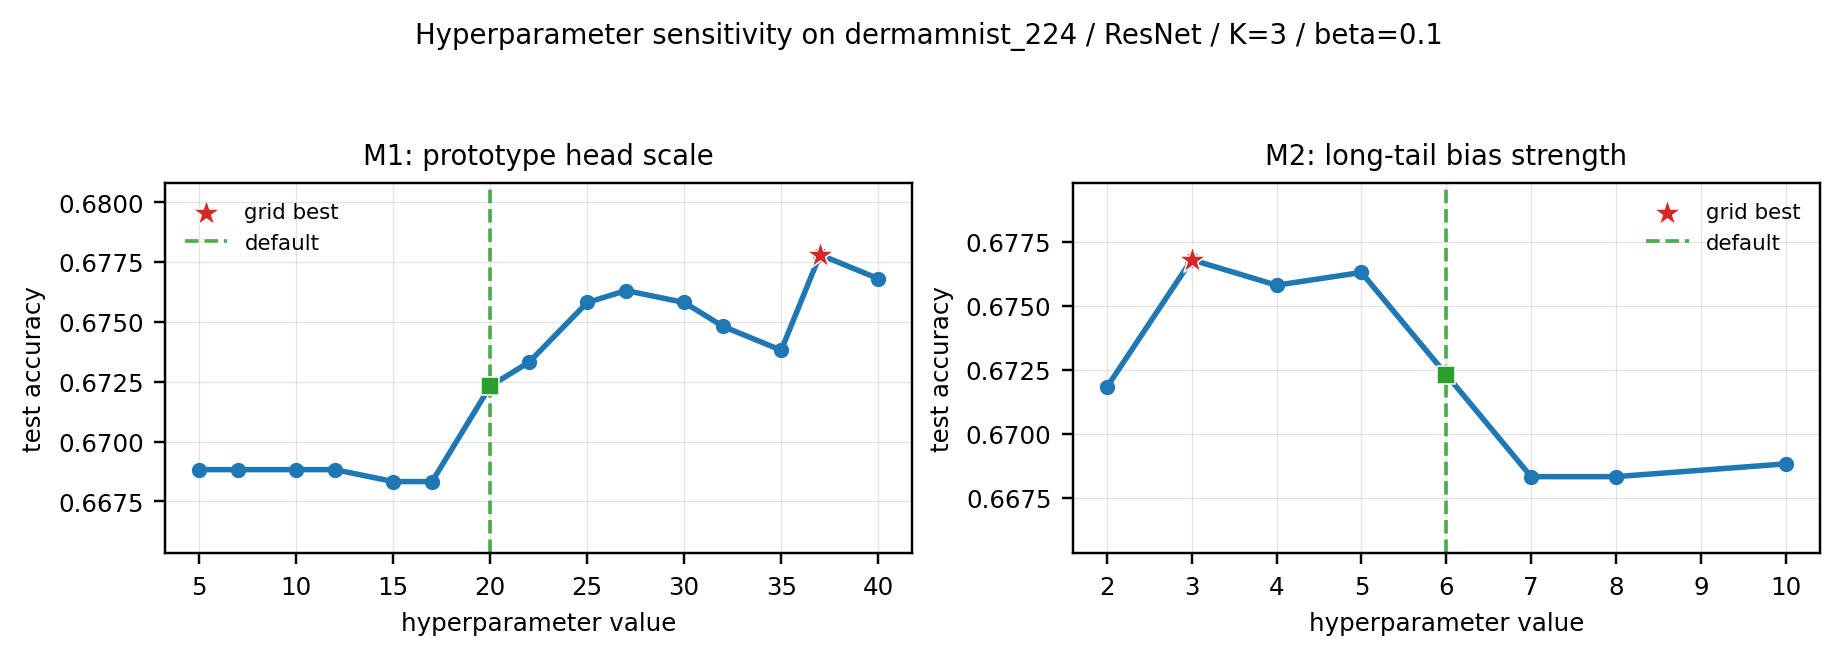
\includegraphics[width=\linewidth]{../figures/lamp_merge_hparam_sensitivity.png}
\caption{Hyperparameter sensitivity of M1 and M2 on \texttt{dermamnist\_224}/ResNet/$K=3$/$\beta=0.1$. Red stars denote grid-best values and green dashed lines denote the default values used by the formal method.}
\label{fig:hparam-sensitivity}
\end{figure}

Figure~\ref{fig:hparam-sensitivity} visualizes the same grid as Table~\ref{tab:hparam-summary}. The default M1 scale and M2 bias strength lie in the high-accuracy plateau, while excessively strong M2 calibration slightly degrades accuracy. This supports treating prevalence calibration as a bounded correction rather than an unrestricted majority-class prior.

\section{V CONCLUSION}

We studied one-shot asynchronous medical model merging, where independently trained hospital models must be fused without federated optimization rounds and without exposing raw medical images to the server. Our empirical analysis shows that generic post-hoc merging methods suffer from aggregation-induced predictive collapse under incomplete local diagnostic coverage. We further show that this collapse can be masked by raw accuracy on long-tailed medical datasets, motivating evaluation with macro recall, macro F1, and prediction-distribution diagnostics.

LAMP-Merge addresses these two properties with a concise two-module design. M1 reconstructs a class-wise diagnostic prototype head from client-side class prototypes in a shared reference feature space, preserving local evidence for each diagnosis class. M2 applies bounded prevalence calibration when uploaded class counts indicate a strongly long-tailed medical prior. Across five medical datasets and five backbone families, LAMP-Merge wins or ties the strongest non-LAMP baseline in 68 out of 75 client-average cells, while also improving balanced accuracy, macro F1, collapse ratio, and effective predicted classes in the diagnostic analysis. These results indicate that medical class-level statistics provide a practical and privacy-preserving signal for asynchronous clinical model fusion.
